\documentclass[tikz]{standalone}
\begin{document}
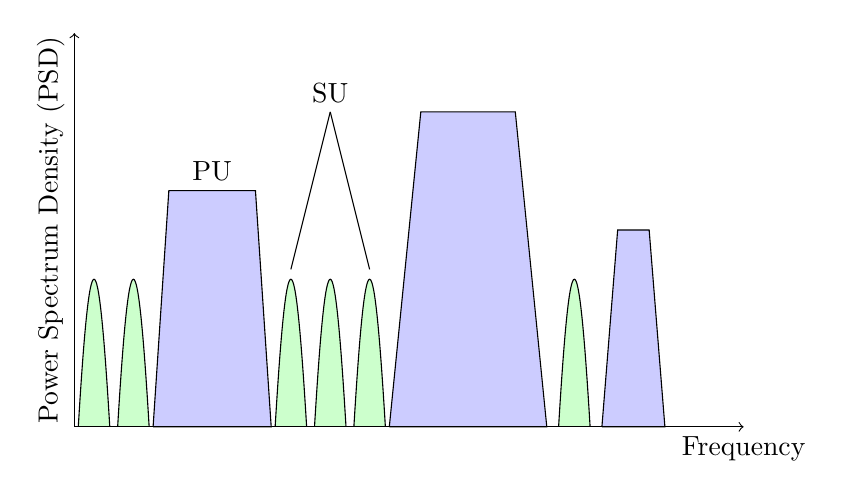
\begin{tikzpicture}
	\draw[fill=blue!20](1,0)--(1.2,3)--node[above]{PU}(2.3,3)--(2.5,0)--(1,0);
	\draw[fill=blue!20](4,0)--(4.4,4)--(5.6,4)--(6,0)--(4,0);
	\draw[fill=blue!20](6.7,0)--(6.9,2.5)--(7.3,2.5)--(7.5,0)--(6.7,0);
	\draw[fill=green!20](0.05,0)..controls(0.2,2.5)and(0.3,2.5)..(0.45,0);
	\draw[fill=green!20](0.55,0)..controls(0.7,2.5)and(0.8,2.5)..(0.95,0);
	\draw[fill=green!20](2.55,0)..controls(2.7,2.5)and(2.8,2.5)..(2.95,0); 
	\draw[fill=green!20](3.05,0)..controls(3.2,2.5)and(3.3,2.5)..(3.45,0);
	\draw[fill=green!20](3.55,0)..controls(3.7,2.5)and(3.8,2.5)..(3.95,0);
	\draw[fill=green!20](6.15,0)..controls(6.3,2.5)and(6.4,2.5)..(6.55,0);
	\draw(2.75,2)--(3.25,4)node[above]{SU};
	\draw(3.25,4)--(3.75,2);
	\draw[->](0,0)--(8.5,0)node[below]{Frequency};
	\draw[->](0,0)--node[above,rotate=90]{Power Spectrum Density (PSD)}(0,5);
\end{tikzpicture}
\end{document}